\documentclass[]{article}
\usepackage[utf8]{inputenc}
\usepackage{graphicx} 

\title{On Contact with the Wizarding World}
\author{Phillip D. Student}
\date{\today}
 
\begin{document}
 
\maketitle % This line make the title show up at the beginning of your document
 
\begin{abstract}
The failure of world governments to make contact with the wizarding world, or rather the wizarding world's continued ability to shield themselves from us, has long stifled international development and induced tensions between non-magic users (so called ``muggles") and those with magic capabilities.
The work in this thesis explores methods that could potentially be exploited for removing the barrier that has been so carefully constructed to separate these two societies, by study of sources detailing life in the wizarding world.
The work in this thesis builds off the studies of Rowling, J. K; Lewis, C. S.; and Tolkien, J.R.R in it's investigation into the origin of the magic world and potential avenues to make contact.
\end{abstract}

\section{Benefits of Magic} \label{sec:BenefitsOfMagic}
In this section we consider some of the benefits that having access to magic would bring on mankind.

\subsection{Benefits of Magical Animals} \label{sec:Animals}
There are several magical animals that are yet undiscovered \cite{rowling2001fantastic} that could provide huge boons to our everyday lifestyle and working environment.
Oliphaunts \cite{tolkien2012lord} have the potential to eliminate the need for heavy construction machinery and heavy-goods transport, and provide little to no air pollution as an additional benefit.
Indeed, we can even predict the resulting pattern in the concentration of carbon dioxide in the atmosphere ($c_{atm}$) on a timescale of years ($t$) after this switch:
\begin{equation} \label{eq:CO2Reduction}
    c_{atm} = c_{0} e^{-\sigma t},
\end{equation}
where $c_{0}$ is the current concentration of carbon dioxide in the atmosphere and $\sigma>0$ is the so-called ``Oliphaunt efficiency coefficient". \newline

Phoenixes, with their healing ability and ease of flight, could effectively act quickly to prevent disaster in environmental crises.
Indeed these remarkable healing properties were discussed in a recent work \cite{graham2019anatomy} which hypothesised how such an ability could have developed through the process of evolution.
\begin{figure}[h]
    \centering
    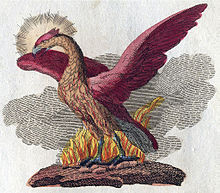
\includegraphics[scale=0.5]{../images/Phoenix_Fabelwesen.jpg}
    \caption{A Phoenix, as depicted by FJ Bertuch. \label{fig:PhoenixFJBertuch}}
\end{figure}
Plus their natural bravery could be used to improve moral in such situations.
Indeed there have been many images depicting their natural bravery and heroism, such as that in figure \ref{fig:PhoenixFJBertuch} illustrated by F.J. Bertuch.

\section{Socio-Economic Considerations}
In this section we will explore some of the social and economic considerations that governments should discuss prior to making contact with the wizarding world.

\subsection*{On Responsible Use of Magic}
With great power comes great responsibility, and so it is only natural that the general population should be subject to a vetting process before being granted access to magical abilities and training \cite{lewis2001chronicles}.
In turn we should ensure that governments are not dominated by magic-using and muggle faction splits, else we create the very divide in society that we are working so hard to eliminate.

\subsection*{On Global Trade and Industry} 
With the ability to apparate, several industries will be negatively impacted.
Commercial travel will be particularly affected, with predictions of up to 95\% loss of gross capital.
In turn the oil and gas industries will suffer from the decreased demand for commercially available fuel, but may benefit substantially from use of the alchemical craft to ``go greener", so to speak.
In particular, in section \ref{sec:Animals} we highlighted some of the beneficial impacts of oliphaunts.
In particular we demonstrated that the concentration of carbon dioxide in the atmosphere would evolve according to equation \ref{eq:CO2Reduction}; inserting our predicted values for $\sigma$ and reported values for $c_{0}$ yields the conclusion that global carbon dioxide levels will fall to pre-industrial levels in as few as 7.5 years.

\bibliographystyle{unsrt}
\bibliography{referencing_example_bib.bib}

\end{document}